\documentclass{article}
\usepackage[utf8]{inputenc}
\usepackage{longtable}
\usepackage{authblk}
\usepackage{adjustbox}
\usepackage{natbib}
\usepackage{lmodern}
\usepackage[T1]{fontenc}
\usepackage[spanish,activeacute]{babel}


\title{\'INDICES DE DESARROLLO HUMANO DE COLOMBIA}

\author[1]{\normalsize Mar\'ia Ang\'elica Galezzo Mart\'inez}
\affil[1]{\small  Escuela de Ingenier\'ia,Universidad de los Andes,\\

\texttt{{ma.galezzo}@uniandes.edu.co}}

\date{30 de junio de 2018}

\usepackage{Sweave}
\begin{document}
\Sconcordance{concordance:Proyecto_final.tex:Proyecto_final.Rnw:%
1 20 1 1 0 20 1 1 5 1 4 14 0 1 2 8 1 1 29 1 4 7 1 1 25 1 3 8 1 1 5 12 0 %
1 2 1 1 1 6 13 0 2 2 4 1 1 3 1 2 8 1 1 5 1 4 31 0 1 2 9 1 1 10 1 13 3 1 %
1 14 1 3 8 1}


\maketitle

\begin{abstract}
Este trabajo eval\'ua el comportamiento del \'Indice de Desarrollo Humano en Colombia con relaci\'on a la poblaci\'n en las cabeceras y en las zonas rurales del pa\'is. Este trabajo eval\'ua el comportamiento del \'Indice de Desarrollo Humano en Colombia con relaci\'on a la poblaci\'on en las cabeceras y en las zonas rurales del pa\'is. Este trabajo eval\'ua el comportamiento del \'Indice de Desarrollo Humano en Colombia con relaci\'on a la poblaci\'on en las cabeceras y en las zonas rurales del pa\'is.Este trabajo eval\'ua el comportamiento del \'Indice de Desarrollo Humano en Colombia con relaci\'on a la poblaci\'on en las cabeceras y en las zonas rurales del pa\'is.
\end{abstract}

\section*{Introducci\'on}

El \'Indide de Desarrollo humano (IDH) es un indicador del desarrollo humano de un pa\'is, el cual tiene en cuenta las dimensiones fundamentales del desarrollo humano, entre ellas: una vida larga y saludeable, adquirir conocimientos fundamentales del desarrollo humano y disfrutar de un nivel de vida digno.El \'indice es el resultado de la media aritm\'etica de los \'indices normalizados de cada una de las dimensiones mencionadas. El \'Indide de Desarrollo humano (IDH) es un indicador del desarrollo humano de un pa\'is, el cual tiene en cuenta las dimensiones fundamentales del desarrollo humano, entre ellas: una vida larga y saludeable, adquirir conocimientos fundamentales del desarrollo humano y disfrutar de un nivel de vida digno.El \'Indice es el resultado de la media aritm\'etica de los <U+00ED>ndices normalizados de cada una de las dimensiones mencionadas. El \'Indide de Desarrollo humano (IDH) es un indicador del desarrollo humano de un pa\'is, el cual tiene en cuenta las dimensiones fundamentales del desarrollo humano, entre ellas: una vida larga y saludeable, adquirir conocimientos fundamentales del desarrollo humano y disfrutar de un nivel de vida digno. 

Comencemos viendo que hay en la secci\'on \ref{univariada} en la p\'agina \pageref{univariada}.

\clearpage

\section {Exploraci\'on Univariada}\label{univariada}

En esta secci\'on se explora el \'indice de desarrollo humano, la poblaci\'on en las cabeceras y  resto del pa\'is para cada uno de los departamentos de Colombia. En esta secci\'on se explora el \'indice de desarrollo humano, la poblaci\'on en las cabeceras y  resto del pa\'is para cada uno de los departamentos de Colombia.En esta secci\'on se explora el \'indice de desarrollo humano, la poblaci\'on en las cabeceras y  resto del pa\'is para cada uno de los departamentos de Colombia.En esta secci\'on se explora el \'indice de desarrollo humano, la poblaci\'on en las cabeceras y  resto del pa\'is para cada uno de los departamentos de Colombia.

Ac\'a podemos ver la informaci\'n estad\'istica para Colombia, debido a que es importante saber el valor central. Como los valores son de naturaleza ordinal debemos pedir la {\bf mediana} y otras medidas de posici\'on (como los \emph{cuartiles}, los que no pediremos pues son pocos valores). La mediana de cada variable la mostramos en la Tabla \ref{stats} en la p\'agina \pageref{stats}.
% Table created by stargazer v.5.2.2 by Marek Hlavac, Harvard University. E-mail: hlavac at fas.harvard.edu
% Date and time: Sat, Jun 30, 2018 - 23:30:31
\begin{table}[!htbp] \centering 
  \caption{Medidas estad'isticas} 
  \label{stats} 
\begin{tabular}{@{\extracolsep{5pt}}lcc} 
\\[-1.8ex]\hline 
\hline \\[-1.8ex] 
Statistic & \multicolumn{1}{c}{N} & \multicolumn{1}{c}{Median} \\ 
\hline \\[-1.8ex] 
Poblaci..n.Cabecera & 32 & 717,197 \\ 
Poblaci..n.Resto & 32 & 268,111.5 \\ 
Poblaci..n.Total & 32 & 1,028,429 \\ 
\hline \\[-1.8ex] 
\end{tabular} 
\end{table} 
Ac\'a podemos ver la informaci\'on estad\'istica para Colombia, debido a que es importante saber el valor central.Ac\'a podemos ver la informaci\'on estad\'istica para Colombia, debido a que es importante saber el valor central.Ac\'a podemos ver la informaci\'on estad\'istica para Colombia, debido a que es importante saber el valor central.Ac\'a podemos ver la informaci\'on estad\'istica para Colombia, debido a que es importante saber el valor central.Ac\'a podemos ver la informaci\'on estad\'istica para Colombia, debido a que es importante saber el valor central.Ac\'a podemos ver la informaci\'on estad\'istica para Colombia, debido a que es importante saber el valor central.Ac\'a podemos ver la informaci\'on estad\'istica para Colombia, debido a que es importante saber el valor central.


Ac\'a podemos observar el histograma del IDH para Colombia \ref{histogramas} en la p\'agina \pageref{histogramas}. 

\begin{figure}[h]
\centering
\begin{adjustbox}{width=12cm,height=7cm,clip,trim=0cm 0.0cm 0cm 0cm}
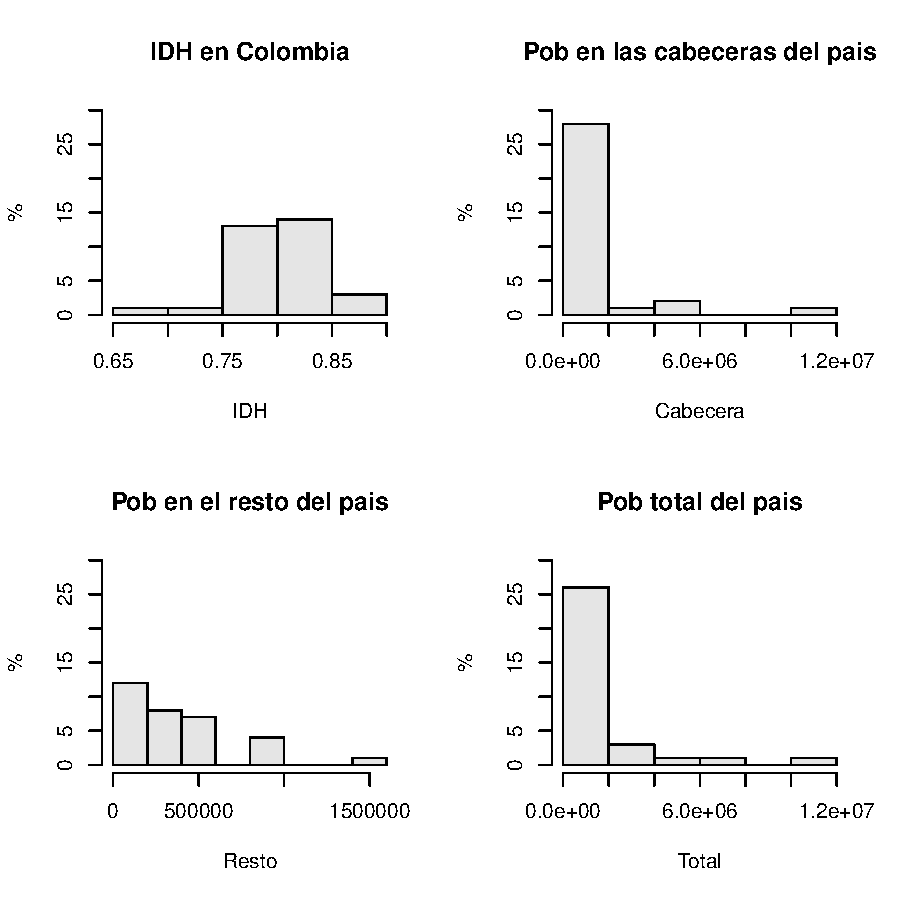
\includegraphics{Proyecto_final-HistogramaIDHPlot}
\end{adjustbox}
\caption{Histogramas}
\label{histogramas}
\end{figure}

\begin{figure}[h]
\centering
\begin{adjustbox}{width=12cm,height=6cm,clip,trim=0cm 0cm 0cm 0cm}
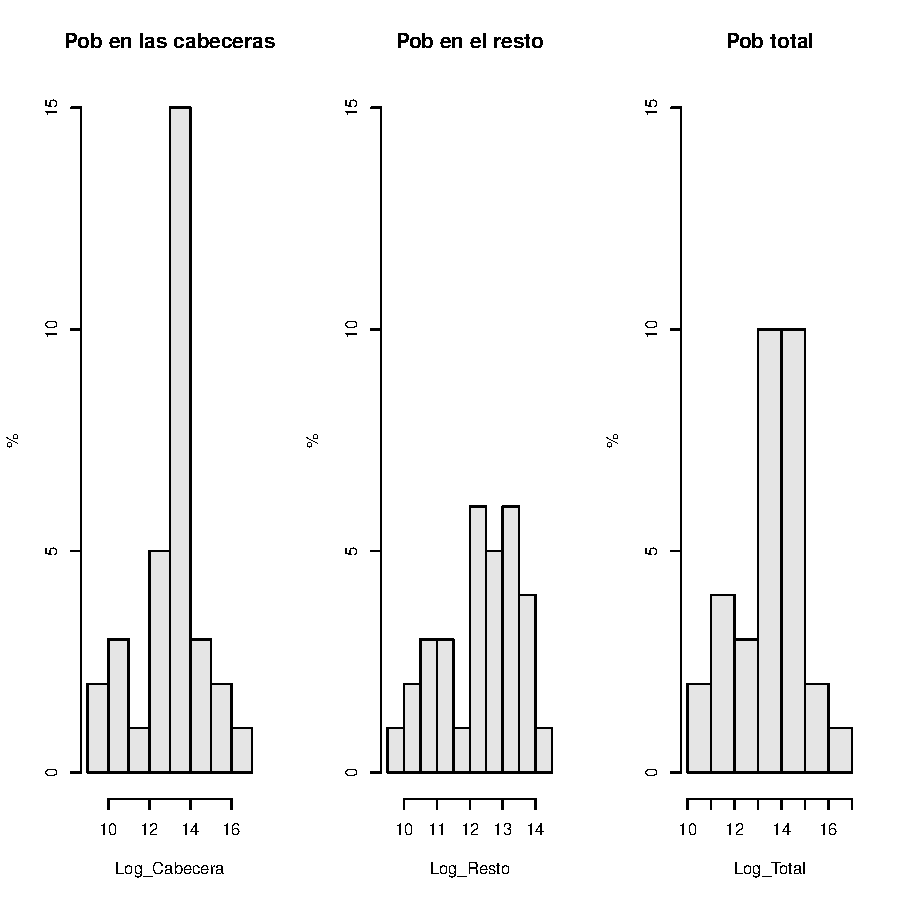
\includegraphics{Proyecto_final-HistogramaIDHNormPlot}
\end{adjustbox}
\caption{Histogramas Normalizados}
\label{histogramas_normalizados}
\end{figure}
\clearpage

\section{Exploraci\'on Bivariada}

En este trabajo se pretende conocer el impacto que tiene la poblaci\'on en el \'Indice de Desarrollo Humano del pa\'is.
% Table created by stargazer v.5.2.2 by Marek Hlavac, Harvard University. E-mail: hlavac at fas.harvard.edu
% Date and time: Sat, Jun 30, 2018 - 23:30:31
\begin{table}[!htbp] \centering 
  \caption{Correlaci'on de IDH con las dem'as variables} 
  \label{} 
\begin{tabular}{@{\extracolsep{5pt}} cc} 
\\[-1.8ex]\hline 
\hline \\[-1.8ex] 
cabeLog & restoLog \\ 
\hline \\[-1.8ex] 
$0.487$ & $0.177$ \\ 
\hline \\[-1.8ex] 
\end{tabular} 
\end{table} 
Veamos la correlaci\'on entre las variables independientes.
% Table created by stargazer v.5.2.2 by Marek Hlavac, Harvard University. E-mail: hlavac at fas.harvard.edu
% Date and time: Sat, Jun 30, 2018 - 23:30:31
\begin{table}[!htbp] \centering 
  \caption{Correlaci'on entre variables independientes} 
  \label{} 
\begin{tabular}{@{\extracolsep{5pt}} ccc} 
\\[-1.8ex]\hline 
\hline \\[-1.8ex] 
 & cabeLog & restoLog \\ 
\hline \\[-1.8ex] 
cabeLog & 1 &  \\ 
restoLog & 0.84 & 1 \\ 
\hline \\[-1.8ex] 
\end{tabular} 
\end{table} \label{corrTable}
Lo visto en la Tabla \ref{corrTable} se refuerza claramente en la Figura \ref{corrPlot}.

\begin{figure}[h]
\centering
\begin{adjustbox}{width=7cm,height=7cm,clip,trim=0cm 0cm 0cm 0cm}
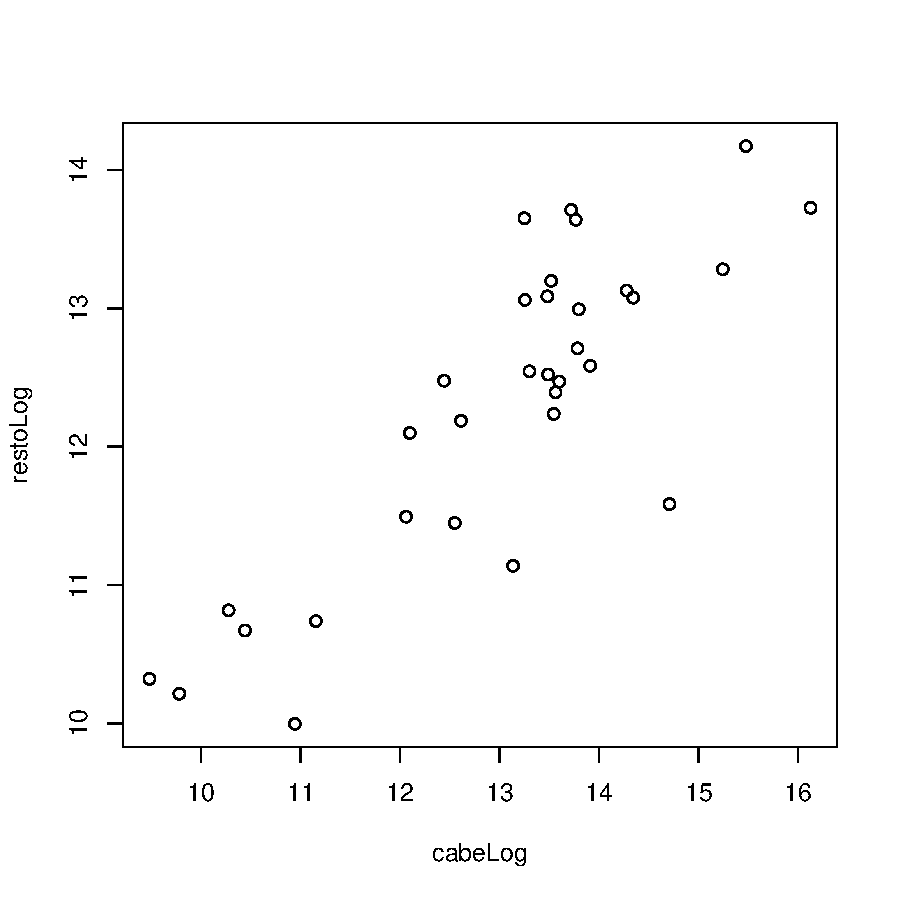
\includegraphics{Proyecto_final-corrPlot}
\end{adjustbox}
\caption{correlaci\'on entre predictores}
\label{corrPlot}
\end{figure}
\clearpage

\section{Modelos de Regresi\'on}
Finalmente, observamos los modelos propuestos, primero sin la poblaci\'on del resto del pa\'is como independiente. Los resultados se muestran en la Tabla \ref{regresiones} de la p\'agina \pageref{regresiones}.


% Table created by stargazer v.5.2.2 by Marek Hlavac, Harvard University. E-mail: hlavac at fas.harvard.edu
% Date and time: Sat, Jun 30, 2018 - 23:30:31
\begin{table}[!htbp] \centering 
  \caption{Modelos de Regresi'on} 
  \label{regresiones} 
\begin{tabular}{@{\extracolsep{5pt}}lcc} 
\\[-1.8ex]\hline 
\hline \\[-1.8ex] 
 & \multicolumn{2}{c}{\textit{Dependent variable:}} \\ 
\cline{2-3} 
\\[-1.8ex] & \multicolumn{2}{c}{IDH} \\ 
\\[-1.8ex] & (1) & (2)\\ 
\hline \\[-1.8ex] 
 cabeLog & 0.013$^{***}$ & 0.031$^{***}$ \\ 
  & (0.004) & (0.007) \\ 
  & & \\ 
 restoLog &  & $-$0.030$^{***}$ \\ 
  &  & (0.010) \\ 
  & & \\ 
 Constant & 0.634$^{***}$ & 0.766$^{***}$ \\ 
  & (0.055) & (0.065) \\ 
  & & \\ 
\hline \\[-1.8ex] 
Observations & 32 & 32 \\ 
R$^{2}$ & 0.238 & 0.425 \\ 
Adjusted R$^{2}$ & 0.212 & 0.385 \\ 
Residual Std. Error & 0.037 (df = 30) & 0.033 (df = 29) \\ 
F Statistic & 9.347$^{***}$ (df = 1; 30) & 10.706$^{***}$ (df = 2; 29) \\ 
\hline 
\hline \\[-1.8ex] 
\textit{Note:}  & \multicolumn{2}{r}{$^{*}$p$<$0.1; $^{**}$p$<$0.05; $^{***}$p$<$0.01} \\ 
\end{tabular} 
\end{table} \clearpage

\section{Exploraci\'on Espacial}

Como acabamos de ver en la Tabla \ref{regresiones} en la p\'agina \pageref{regresiones}, si quisieras sintetizar la multidimensionalidad de nuestros indicadores, podr\'iamos usar tres de las cuatro variables que tenemos (un par de las originales tiene demasiada correlaci\'on). 

As\'i, propongo que calculemos conglomerados de pa\'ises usando toda la informaci\'on de tres de los indicadores. Como nuestras variables son ordinales utilizaremos un proceso de conglomeraci\'on donde las distancia ser\'an calculadas usando la medida {\bf gower} propuestas en \cite{macqueen_methods_nodate}. Los tres conglomerados se muestran en la Figura \ref{clustmap}.

Estos son los lugares donde tenemos informaci\'on:



\begin{figure}[h]
\centering
\begin{adjustbox}{width=10cm,height=8cm,clip,trim=1cm 1cm 1cm 1cm}
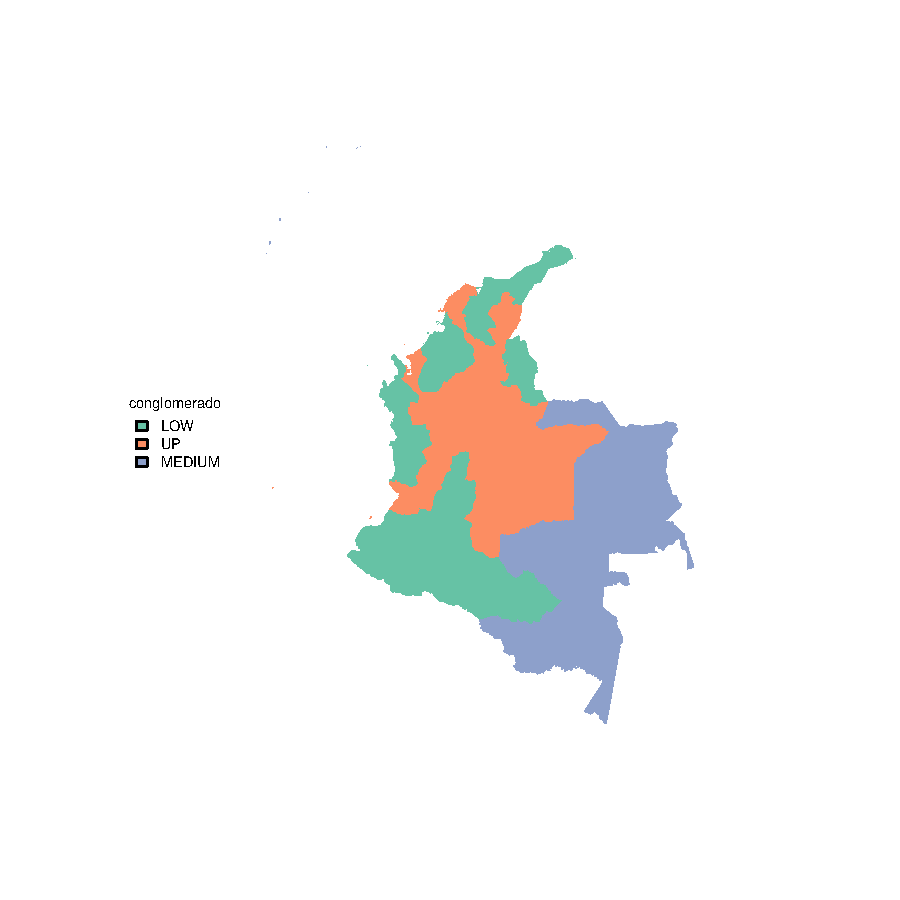
\includegraphics{Proyecto_final-plotMap}
\end{adjustbox}
\caption{Conglomerado de departamentos seg\'un sus indicadores de desarrollo humano}\label{clustmap}
\end{figure}
\clearpage
\bibliographystyle{abbrv}
\renewcommand{\refname}{Bibliograf\'ia}
\bibliography{IDH}

\end{document}
